\documentclass{article}

\usepackage{amsmath,amssymb}
\usepackage{multicol}
\usepackage{systeme}
\usepackage{url}
%\usepackage{siunitx}

% for drawing graphs
\usepackage{tikz}
\tikzset{every picture/.style={thick}}
\tikzset{every node/.style={draw, circle, inner sep = 2pt}}
\usetikzlibrary{arrows}

% for margins
\usepackage[margin=1in]{geometry}

% for font
\usepackage{euler}
\usepackage[OT1]{eulervm}
\renewcommand{\rmdefault}{pplx}

\setlength{\parindent}{0pt}  %no indenting

% MACROS
\newcommand{\trans}{^\top}
\newcommand{\adj}{^{\rm adj}}
\newcommand{\cof}{^{\rm cof}}
\newcommand{\inp}[2]{\left\langle#1,#2\right\rangle}
\newcommand{\dunion}{\mathbin{\dot\cup}}
\newcommand{\bzero}{\mathbf{0}}
\newcommand{\bone}{\mathbf{1}}
\newcommand{\ba}{\mathbf{a}}
\newcommand{\bb}{\mathbf{b}}
\newcommand{\bd}{\mathbf{d}}
\newcommand{\be}{\mathbf{e}}
\newcommand{\bp}{\mathbf{p}}
\newcommand{\bq}{\mathbf{q}}
\newcommand{\bx}{\mathbf{x}}
\newcommand{\by}{\mathbf{y}}
\newcommand{\bz}{\mathbf{z}}
\newcommand{\bu}{\mathbf{u}}
\newcommand{\bv}{\mathbf{v}}
\newcommand{\bw}{\mathbf{w}}
\newcommand{\tr}{\operatorname{tr}}
\newcommand{\nul}{\operatorname{null}}
\newcommand{\rank}{\operatorname{rank}}
%\newcommand{\ker}{\operatorname{ker}}
\newcommand{\range}{\operatorname{range}}
\newcommand{\Col}{\operatorname{Col}}
\newcommand{\Row}{\operatorname{Row}}
\newcommand{\spec}{\operatorname{spec}}
\newcommand{\vspan}{\operatorname{span}}
% \newenvironment{sol}{\medskip\noindent {\bf Solution.}}{\newpage}
\newcommand{\mystrut}{\rule[-.5\baselineskip]{0pt}{2\baselineskip}}
% \newcommand{\mul}{\operatorname{mul}}
\newcommand{\even}{\operatorname{even}}
\newcommand{\sgn}{\operatorname{sgn}}
\newcommand{\iner}{\operatorname{iner}}
\newcommand{\rL}{\mathring{L}}
\newcommand{\diag}{\operatorname{diag}}

\makeatletter
%%%The definition of \binom is \genfrac ()\z@ {}
%%%To adjust the spaces between parantheses, change the augment of \kern
\newcommand{\multiset}[2]{\ensuremath{\left(\kern-.3em\left(\genfrac{}{}{\z@}{}{#1}{#2}\right)\kern-.3em\right)}}
\newcommand{\qanalog}[2]{\genfrac []\z@ {}{#1}{#2}_q}
\makeatother

% for title
\title{2021F Math585 Midterm 2}
\date{\vspace{-1cm}}
\begin{document}
\maketitle
\large

\textbf{5 questions}, \textbf{$20(+5)$ total points}

\textbf{Note:}  Use other papers to answer the problems.  Remember to write down your \textbf{name} and your \textbf{student ID \#}.

\begin{enumerate}
\setlength\itemsep{2em}

\item{} [5pt] Let $G$ be the graph below and $A$ its adjacency matrix.  Find $\rank(A)$ and $\det(A)$.

\begin{center}
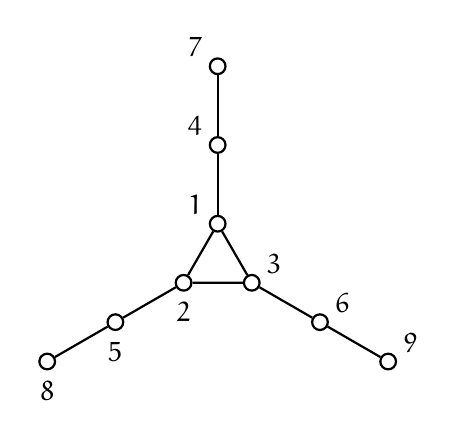
\begin{tikzpicture}
\foreach \i in {1,2,3} { 
\pgfmathsetmacro{\ang}{90 + 120*(\i - 1)}
\pgfmathsetmacro{\angr}{\ang + 60}
\pgfmathsetmacro{\ip}{int(\i + 3)}
\pgfmathsetmacro{\ipp}{int(\i + 6)}
\node[label={\angr:$\i$}] (\i) at (\ang:0.5) {};
\node[label={\angr:$\ip$}] (\ip) at (\ang:1.5) {};
\node[label={\angr:$\ipp$}] (\ipp) at (\ang:2.5) {};
\draw (\i) -- (\ip) -- (\ipp);
}
\draw (1) -- (2) -- (3) -- (1);
\end{tikzpicture}
\end{center}

\item{} [5pt] Let $G$ be a graph and $A$ its adjacency matrix.  Suppose the characteristic polynomial of $A$ is 
\[(-x)^5 -4(-x)^3 + 2(-x).\]
Find $G$.

\item{} [5pt] Let $G$ be a graph and $A$ its adjacency matrix.  Suppose $G$ is a graph containing an induced subgraph that is isomorphic to $K_k$.  Prove that $A$ has at least $k - 1$ eigenvalues that are at most $-1$.

\vfill

\textbf{Two more problems on the back.}

\newpage
\item{} [5pt] Let $G$ be the graphs below and $A$ its adjacency matrix.  

\begin{center}
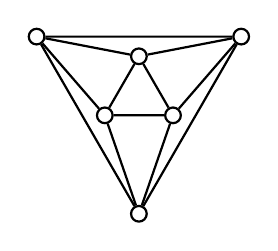
\begin{tikzpicture}
\foreach \i in {1,2,3} { 
\pgfmathsetmacro{\ang}{90 + 120*(\i - 1)}
\pgfmathsetmacro{\angr}{30 + 120*(\i - 1)}
\pgfmathsetmacro{\ip}{int(\i + 3)}
\node (\i) at (\ang:0.5) {};
\node (\ip) at (\angr:1.5) {};
}
\draw (1) -- (2) -- (3) -- (1);
\draw (4) -- (5) -- (6) -- (4);
\draw (1) -- (5) -- (2) -- (6) -- (3) -- (4) -- (1);
\end{tikzpicture}
\end{center}
Find the eigenvalues of $A$.

\item{} [extra 5pt] Let 
\[A = \begin{bmatrix}
 O & B & O \\
 O & O & C \\
 D & O & O 
\end{bmatrix},\]
where $O$ is the $3\times 3$ zero matrix and $B$, $C$, $D$ are some fixed $3\times 3$ matrices.  Let $\omega = e^{i\frac{2\pi}{3}}$.  Show that if $\lambda$ is an eigenvalue of $A$, then $\omega\lambda$ is also an eigenvalue of $A$.

\end{enumerate}



\end{document}



  
